%
% template.tex -- slide template
%
% (c) 2021 Prof Dr Andreas Müller, OST Ostschweizer Fachhochschule
%
\bgroup
\begin{frame}[t]
\setlength{\abovedisplayskip}{5pt}
\setlength{\belowdisplayskip}{5pt}
\frametitle{Zusammenhang}
\vspace{-20pt}
\begin{columns}[t,onlytextwidth]
\begin{column}{0.48\textwidth}
\begin{block}{Zusammenhängend --- oder nicht}
\begin{center}
\begin{tikzpicture}[>=latex,thick]
\def\ds{2.4}
\coordinate (A) at (0,0);
\coordinate (B) at (\ds,0);
\coordinate (C) at ({2*\ds},0);

\node at (A) {$\operatorname{SO}(n)$};
\node at (B) {$\operatorname{O}(n)$};
\node at (C) {$\{\pm 1\}$};

\draw[->,shorten <= 0.6cm,shorten >= 0.5cm] (A) -- (B);
\draw[->,shorten <= 0.5cm,shorten >= 0.5cm] (B) -- (C);
\node at ($0.5*(B)+0.5*(C)$) [above] {$\det$};

\coordinate (A2) at (0,-1.0);
\coordinate (B2) at (\ds,-1.0);
\coordinate (C2) at ({2*\ds},-1.0);

\draw[color=blue] (A2) ellipse (1cm and 0.3cm);
\draw[color=blue] (B2) ellipse (1cm and 0.3cm);
\node[color=blue] at (C2) {$+1$};

\coordinate (A3) at (0,-1.7);
\coordinate (B3) at (\ds,-1.7);
\coordinate (C3) at ({2*\ds},-1.7);

\draw[->,shorten <= 1.1cm,shorten >= 0.3cm] (B2) -- (C2);
\draw[->,shorten <= 1.1cm,shorten >= 0.3cm] (B3) -- (C3);

\draw[color=red] (B3) ellipse (1cm and 0.3cm);
\node[color=red] at (C3) {$-1$};

\end{tikzpicture}
\end{center}
\end{block}
\begin{block}{Zusammenhangskomponente von $e$}
$G_e\subset G$ grösste zusammenhängende Menge, die $e$ enthält:
\begin{align*}
\operatorname{SO}(n)&\subset \operatorname{O}(n)
\\
\{A\in\operatorname{GL}_n(\mathbb{R})\,|\, \det A > 0\}
	&\subset \operatorname{GL}_n(\mathbb{R})
\end{align*}
\end{block}
\end{column}
\begin{column}{0.48\textwidth}
\begin{block}{Eigenschaften}
\begin{itemize}
\item
{\bf Untergruppe}: $\gamma_i(t)$ Weg von $e$ nach $g_i$,
dann ist
\begin{itemize}
\item
$\gamma_1(t)\gamma_2(t)$ ein Weg von $e$ nach $g_1g_2$
\item
$\gamma_1(t)^{-1}$ Weg von $e$ nach $g_1^{-1}$
\end{itemize}
\item
{\bf Normalteiler}: $\gamma(t)$ ein Weg von $e$ nach $g$, dann 
ist $h\gamma(t)h^{-1}$ ein Weg von $h$ nach $hgh^{-1}$
$\Rightarrow hG_eh^{-1}\subset G_e$
\end{itemize}
\end{block}
\begin{block}{Quotient}
$G/G_e$ ist eine diskrete Gruppe
\begin{center}
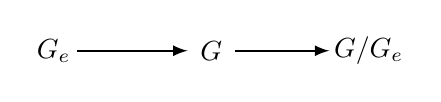
\begin{tikzpicture}[>=latex,thick]
\coordinate (A) at (0,0);
\coordinate (B) at (2,0);
\coordinate (C) at (4,0);
\node at (A) {$G_e$};
\node at (B) {$G$};
\node at (C) {$G/G_e$};
\draw [->,shorten <= 0.3cm,shorten >= 0.3cm] (A) -- (B);
\draw [->,shorten <= 0.3cm,shorten >= 0.5cm] (B) -- (C);
\end{tikzpicture}
\end{center}
\vspace{-7pt}
$\Rightarrow$ $G_e$ und $G/G_e$ separat studieren
\end{block}
\end{column}
\end{columns}
\end{frame}
\egroup
